
\section{개론}

n차 다항식 $A(x)$를 예시로 들라고하면 대부분 이렇게 대답할것이다.

$$A(x) = a_0x^0 + a_1x^1 + a_2x^2 + \cdots + a_{n}x^n = \sum_{k=0}^{n} a_kx^k$$

이는 컴퓨터상에서 크기가 $n+1$인 벡터(배열)에 $\left\{a_0,a_2, ... , a_n \right\}$으로 나타내도 $A(x)$를 확정지을 수 잇다. 이러한 표현 방식을 \textbf{계수 표현(Coefficient representation)}이라고 한다.
우리 일반적으로 사용하는 다항식을 나타내는 방식이라고 생각하면되는데. 
이렇게 나타낸 다항식을 각각 곱하는 경우를 생각해보자.
일반적으로 우리는 종이에서 다음 다항식을 곱할때 이와같이 풀것이다.

$$C(x) = A(x)B(x) = (a_0x^0 + a_1x^1 + a_2x^2 + \cdots + a_nx^n)(b_0x^0 + b_1x^1 + b_2x^2 + \cdots + b_nx^n)$$

2차나 3차의 경우는 한번에 쭉 풀수도있겠지만
n이 큰 경우일때는 어쩔수없이 $A(x)$ 항하나에 $B(x)$를 곱해서 쭉 전개해서 풀것이다. 설명의 편의를 위해서 $A(x)$와 $B(x)$의 최고차항의 차수가 같다고 가정하고 내용을 진행할 것이고 전체 흐름에 따라 $n$의 의미가 중구난방적이다.

이를 직접 컴퓨터에서 계산한다고 생각해보자.
벡터 각요소에 벡터 각요소를 각각 모두 곱하기 때문에 시간복잡도는 $O(n^2)$이 될것이다. 이것이 우리가 일반적으로 생각하는 다항식 곱의 시간복잡도이다
이를 $O(n \log n)$으로 줄여 보는 것이 목표이다.

\section{점값 표현}

중,고등학교를 나오면서 다음과 같은 문제를 푼적이 있을거라고 생각한다.

\begin{framed}
    \begin{itemize}
        \item 2차원 좌표상에서 $(1,0)$과 $(6,8)$을 지나는 직선의 방정식을 구하시오.
        \item 2차원 좌표상에서 $(1,0)$, $(6,8)$,$(-4,8)$ 을 지나는 다항함수를 구하시오.
    \end{itemize}
\end{framed}

간단한 연립방정식처럼 생각하면 최고차항의 차수가 $n$에 따라서 어떤 다항식을 지나는 $n+1$개 이상의 점의 좌표를 알고있으면 그 다항식을 특정할 수 있다.
컴퓨터상에서도 그대로 나타낼수 있다.
$\left\{(x_1, y_1),(x_2, y_2), ... ,(x_n, y_n)\right\}$

이를 \textbf{점값 표현(Point-value representation)}이라고 한다.
점값 표현으로 이용할 특징은 같은 좌표의 덧셈과 곱셈은 그냥 단순히 더하고 곱하면되는것이다. 
$C(x) = A(x)B(x)$에 대해서 $A(x_k)*B(x_k) = C(x_k)$가 된다. 따라서 점값표현으로 나타나있는 $A(x)$와 $B(x)$의 다항식 곱을 나타내기위해 $O(n)$의 시간만큼 걸린다. 실제로는 $C(n)$을 특정하기위해서 $2n-1$만큼의 좌표쌍이 필요하다.
그만큼 $A(x), B(x)$의 좌표쌍 또한 $2x-1$개 만큼 필요하다.

\section{계수표현 점값표현 치환에 대한 고찰}
앞에서 점값표현으로 나타냈을때 다항식의 곱이 간편하다는것을 알았다. 이제 계수표현으로 나타나있는 다항식을 점값표현으로 나타내고 이것의 역변환을 빠르게 할 생각을 하면된다.

\begin{enumerate}
    \item $x$좌표를 임의로 잡고 하나씩 계산하는 경우이다.

    그럼 $n+1$개의 계수에 대해서 $x$가 $x^n, ... , x$를 구해서 계수를 각각 계산하는것은 $n + \cdots + 1 = \dfrac{1}{2}n^2 + n$만큼의 시간이 걸린다. 이때 $x$차수를 구하는 부분을 메모이제이션을 사용한다면 $O(2n)$만큼 걸린다.

    \item 호어의 법칙(Horner's rule)
        특정값 $x_0$에 대해 점값표현을 가장 빠르게 구할방법은 연쇄적으로 계산을 하는것이다.
        $A(x_0) = a_0 + x_0(a_1 + x_0(a_2+ \cdots + x_0(a_{n-2} + x_0(a_{n-1})) \cdots ))$
        위 방식에 비해서 추가적인 공간복잡도도 $O(1)$이며 메모리 접근도 적기때문에 훨씬 빠르다고 볼수있다.
        하지만 $n$개의 점값표현을 구하기위해선 결국 $O(n^2)$만큼의 시간이 걸리기때문에 다항식을 쌩으로 곱하는것과 다를것이없다.
\end{enumerate}

\section{DFT와 FFT}
변환과 역변환에 $O(n^2)$으로 푸는 방법까지는 알았다. 
$x$점으로 복소수 근을 가지게 함으로써 변환에 $O(n \log n)$이 걸림을 보일수있다.

\begin{figure}[h!]
%    \centering
    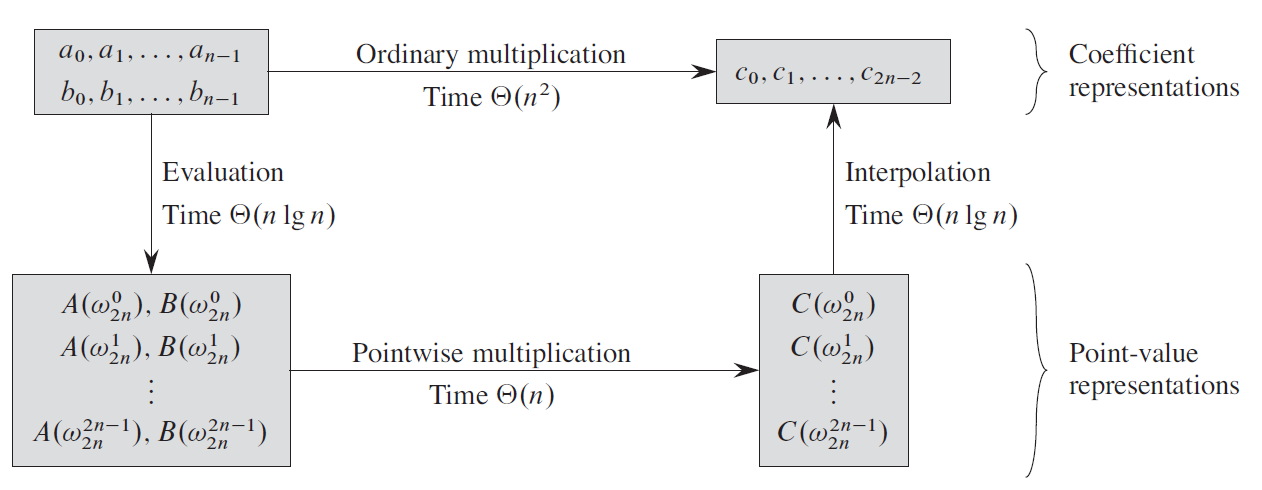
\includegraphics[scale=0.5]{./FFT/pic/pic1.PNG}
    \caption{다항식곱의 전체 알고리즘 개형도}
\end{figure}

전체적인 순서는 이렇게된다.
\begin{enumerate}
    \item $A(x)$와 $B(x)$에 $n~2n$까지의 차수의 계수를 0으로 놓아 벡터를 확장한다.
    \item 각각 FFT를 적용하여 점값표현을 구한다.
    \item 점별로 곱해 $C(x)$를 구한다.
    \item 다시 FFT를 적용하여 $C(x)$를 계수형으로 바꾼다.
\end{enumerate}




\subsection{복소수}
복소수는 오일러 방정식으로 부터 시작합니다.
$e^{ix} = \cos(x) +i\sin(x)$
$x = \pi$를 넣으면 $e^{i\pi} = -1$이란 어디서 봤을 수도있는 식입니다.
여기에 $x = 2\pi$를 넣으면 $e^{2\pi i} = 1$이란 식이 나옵니다. 
이제 $\omega_n$을 다음과 같이 정의합니다.
$\omega_n = e^{\frac{2\pi i}{n}}$ 

$\omega_n$을 $0$부터 $n-1$까지 지수승 한 집합을 나타내자.

$\left\{\omega_n^0,\omega_n^1, ... , \omega_n^{n-1} \right\}$

이는 순환 구조를 나타낸다 
$\omega_n ^0 = \omega_n^n = 1$

우리의 목적은 최고차항이 $n-1$인 다항식의 점값표현으로 쓸 $x$좌표로 다음의 집합을 채택하는것이다.


\begin{figure}[h!]
    \centering
    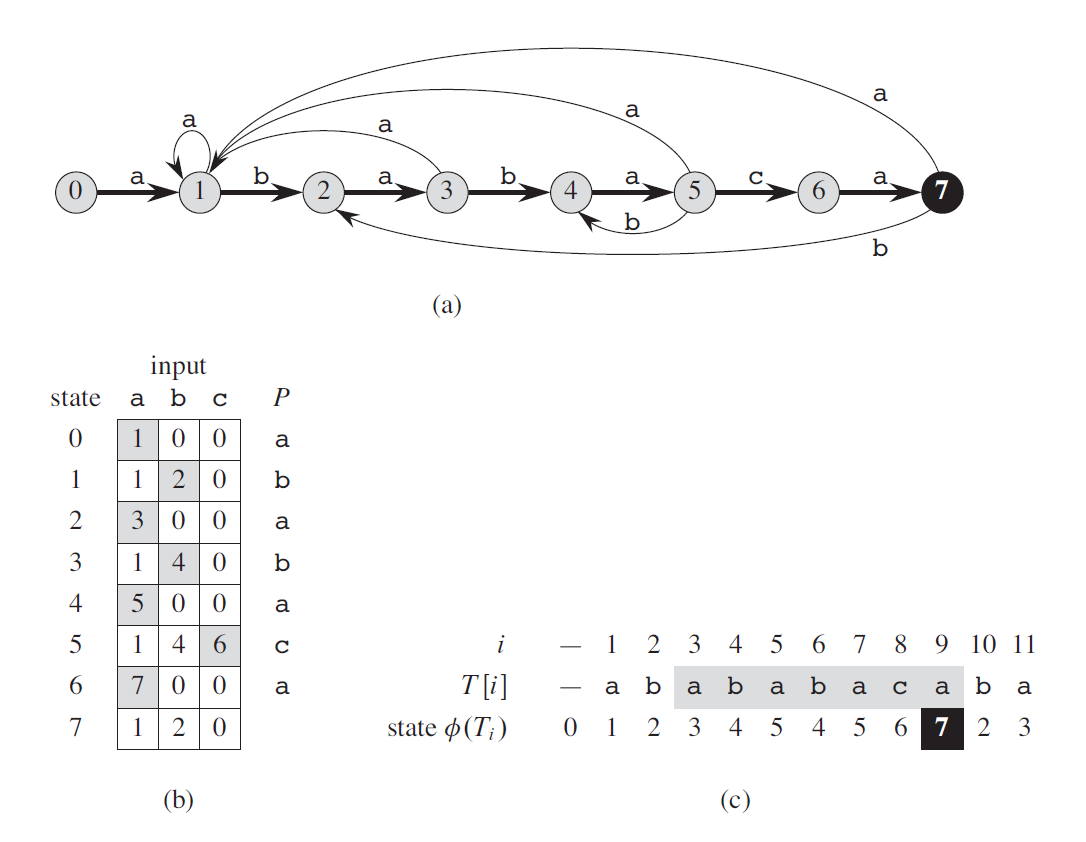
\includegraphics[scale=0.3]{./FFT/pic/pic2.png}
    \caption{단위값의 8번째근}
\end{figure}

\subsection{DFT}

계수형으로 나타나있는 $A(x) = (a_0,a_1,...,a_n)$를 다음 $y = (y_0,y_1,...,y_n) $벡터를 \textbf{이산 푸리에 변환(DFT : Discrete Fourier Transform)}이라한다.

$$ y_k = A(\omega^k_n) = \sum_{j=0}^{n-1} a_j\omega_{n}^{kj}$$

쉽게 나타내면 계수표현으로 나타나 있는 $A(x)$를 n개의 집합이$\left\{\omega_n^1, \omega_n^2 , ... , \omega_n^{n-1}\right\}$인 $x$좌표에 대한 $y$값의 집합입니다.

\subsection{FFT}
DFT를 $O(n \log n)$에 구할수있는 알고리즘으로 \textbf{고속 푸리에 변환(FFT :Fast Fourier Transform)}이 있다. 

FFT는 분할 정복(divide and conquer)기법을 사용하여 나타낼 수 있다.
$A_{even}$과 $A_{odd}$를 다음과 같이 정의한다.
$A_{even}(x) = a_0x^0 + a_2x^1 + a_4x^2 + \cdots + a_{n-2}x^{ \frac{n}{2}-1} $
$A_{odd}(x) = a_1x^0 + a_3x^1 + a_5x^2 + \cdots + a_{n-1}x^{\frac{n}{2}-1} $
$A(x)$를 다음과 같이 분할한다.

$A(x) = A_{even}(x^2) + xA_{odd}(x^2) $

프로시저는 다음과 같다.
\begin{enumerate}
    \item $A_{even}$과 $A_{odd}$로 나눈다.
    \item $A_{even}$과 $A_{odd}$를 각각 재귀로 FFT한다.
    \item $A(x) = A_{even}(x^2) + xA_{odd}(x^2) $에 따라서 계산한다. 이때 걸리는 복잡도는 $O(n)$
\end{enumerate}


%https://www.cs.dartmouth.edu/~thc/clrscode/clrscode3e.pdf
\begin{lstlisting}[style = CStyle]
RECURSIVE_FFT(a)
n = length[a]
if n = 1
    return a
w_n = e ^{2 pi i / n}
w = 1
a_even = (a_0,a_2 , ..., a_n-2)
a_odd = (a_1,a_3 , ..., a_n-1)

y_even = RECURSIVE_FFT(a_even)
y_odd = RECURSIVE_FFT(a_odd)
for( k = 0 to n/2 -1 )
    y[k] = y_even[k] + wy_odd[k]
    y[k+(n/2)] = y_even[k] - wy_odd[k]
    w = w*w_n
return y
\end{lstlisting}

이 알고리즘은 2로 나눈 재귀를 두번부르고 후에 추가적인 O(n)연산이있다.
$T(n) = 2T\left(\dfrac{n}{2}\right) + \Theta(n) = \Theta(n \log n)$

\section{$DFT^{-1}$ 역변환}

점값표현에 대해서 다음의 식이 성립이 한다.

$$ a_j = \dfrac{1}{n}\sum_{k=0}^{n-1} y_k\omega_{n}^{-kj}$$

$DFT$는 다음의 행렬 곱셈 식을 이용했다.

$
\begin{pmatrix}
    y_0 \\ 
    y_1 \\
    y_2 \\
    \vdots \\
    y_{n-1}
\end{pmatrix}
=
\begin{pmatrix}
    1 & 1 & 1 & 1 & \cdots & 1 \\
    1 & \omega_n & \omega_n^2 & \omega_n^3 & \cdots & \omega_n^{n-1} \\
    1 & \omega_n^2 & \omega_n^4 & \omega_n^6 & \cdots & \omega_n^{2(n-1)} \\
    1 & \omega_n^3 & \omega_n^6 & \omega_n^9 & \cdots & \omega_n^{3(n-1)} \\
    \vdots & \vdots & \vdots & \vdots & \ddots & \vdots \\
    1 & \omega_n^{n-1} & \omega_n^{2(n-1)} & \omega_n^{3(n-1)} & \cdots & \omega_n^{(n-1)(n-1)} 
\end{pmatrix}
\begin{pmatrix}
    a_0 \\ 
    a_1 \\
    a_2 \\
    \vdots \\
    a_{n-1}
\end{pmatrix}
$

역행렬이 존재하며, 역변환에 대해서 다음의 식을 통해 원래의 값이 나온다.

$
\begin{pmatrix}
    a_0 \\ 
    a_1 \\
    a_2 \\
    \vdots \\
    a_{n-1}
\end{pmatrix}
= \dfrac{1}{n}
\begin{pmatrix}
    1 & 1 & 1 & 1 & \cdots & 1 \\
    1 & \omega_n^{-1} & \omega_n^{-2} & \omega_n^{-3} & \cdots & \omega_n^{-(n-1)} \\
    1 & \omega_n^{-2} & \omega_n^{-4} & \omega_n^{-6} & \cdots & \omega_n^{-2(n-1)} \\
    1 & \omega_n^{-3} & \omega_n^{-6} & \omega_n^{-9} & \cdots & \omega_n^{-3(n-1)} \\
    \vdots & \vdots & \vdots & \vdots & \ddots & \vdots \\
    1 & \omega_n^{-(n-1)} & \omega_n^{-2(n-1)} & \omega_n^{-3(n-1)} & \cdots & \omega_n^{-(n-1)(n-1)} 
\end{pmatrix}
\begin{pmatrix}
    y_0 \\ 
    y_1 \\
    y_2 \\
    \vdots \\
    y_{n-1}
\end{pmatrix}
$

\section{n = 4 일때 수행 예시}

$e^{i\theta} = \cos \theta + i \sin \theta$

% https://tex.stackexchange.com/questions/34902/what-does-right-do?rq=1


\subsection{$DFT$ 수행}

$
\omega^j = \left\{
\begin{array}{rl}
    1 & ( j = 0, \theta = 0 ) \\
    i & ( j = 1, \theta = \dfrac{1}{2}\pi) \\
    -1 & ( j = 2, \theta = \pi )\\
    -i & ( j = 3, \theta = \dfrac{3}{2}\pi) \\
\end{array}
\right.
$


계수 벡터 $A = \left\{a_0, a_1, a_2, a_3 \right\}$인 경우를 생각해보자. 이를 점값표현으로 변환, 역변환해 본다.

\begin{enumerate}
    \item 분할: $\left\{a_0, a_2 \right\}$, $\left\{a_1, a_3\right\}$
    \item 분할: $\left\{a_0\right\}, \left\{a_2\right\}, \left\{a_1\right\}, \left\{a_3\right\}$
    \item 결합: $\left\{a_0 + a_2, a_0 - a_2 \right\}\left\{a_1 + a_3, a_1 - a_3\right\}$
    \item 결합: $\left\{(a_0 + a_1 + a_2 + a_3), (a_0 + \omega a_1 - a_2 -\omega a_3) , \\(a_0 - a_1 + a_2 - a_3), (a_0 - \omega a_1 - a_2 + \omega a_3) \right\}$
\end{enumerate}

계수벡터에 $1, \omega ,\omega^2 , \omega^3 $을 넣었을때의 결과와 동일하다.

$
\begin{pmatrix}
    y_0 \\ 
    y_1 \\
    y_2 \\
    y_3 
\end{pmatrix}
=
\begin{pmatrix}
    a_0 + a_1 + a_2 + a_3 \\ 
    a_0 + \omega a_1 - a_2 -\omega a_3 \\
    a_0 - a_1 + a_2 - a_3 \\
    a_0 - \omega a_1 - a_2 + \omega a_3
\end{pmatrix}
$


\subsection{$DFT^{-1}$수행}

$
\omega^j = \left\{
\begin{array}{rl}
    1 & ( j = 0, \theta = 0 ) \\
    -i & ( j = -1, \theta = -\dfrac{1}{2}\pi) \\
    -1 & ( j = -2, \theta = -\pi ) \\
    i & ( j = -3, \theta = -\dfrac{3}{2}\pi ) \\
\end{array}
\right.
$


$-\omega = \omega^{-1}$
\footnote{참고: $\cos$은 우함수(y축 대칭) $\sin$은 기함수(원점대칭)이다. }

\begin{enumerate}
    \item 분할: $\left\{y_0, y_2 \right\}$, $\left\{y_1, y_3\right\}$
    \item 분할: $\left\{y_0\right\}, \left\{y_2\right\}, \left\{y_1\right\}, \left\{y_3\right\}$
    \item 결합: $\left\{y_0 + y_2, y_0 - y_2 \right\}\left\{y_1 + y_3, y_1 - y_3\right\}$
    \item 결합: $\left\{(y_0 +y_1 + y_2 + y_3), (y_0 - \omega y_1 + y_2 +\omega y_3) , \\(y_0 - y_1 +y_2 - y_3), (y_0 + \omega y_1 - y_2 - \omega y_3) \right\}$
\end{enumerate}

$
\begin{pmatrix}
    a_0 \\ 
    a_1 \\
    a_2 \\
    a_3 
\end{pmatrix}
= \dfrac{1}{n}
\begin{pmatrix}
    y_0 + y_1 + y_2 + y_3 \\ 
    y_0 - \omega y_1 - y_2 +\omega y_3 \\
    y_0 - y_1 + y_2 - y_3 \\
    y_0 + \omega y_1 - y_2 - \omega y_3
\end{pmatrix}
$


각$y_n$에 곱해지는 계수와 $a_n$ 계수벡터를 풀어써서 행렬에 나타내면


\begin{itemize}
    \item $a_1$
    
    $
        \begin{pmatrix}
            1 & -\omega & -1 & \omega
        \end{pmatrix}
        \begin{pmatrix}
            1 & 1 & 1 & 1 \\
            1 & \omega & -1 & -\omega \\
            1 & -1 & 1 & -1 \\
            1 & -\omega & -1 & \omega 
        \end{pmatrix}
    $
    
    \item $a_2$
    
    $
    \begin{pmatrix}
        1 & -1 & 1 & -1
    \end{pmatrix}
    \begin{pmatrix}
        1 & 1 & 1 & 1 \\
        1 & \omega & -1 & -\omega \\
        1 & -1 & 1 & -1 \\
        1 & -\omega & -1 & \omega 
    \end{pmatrix}
    $
    \item $a_3$
    

    $
    \begin{pmatrix}
        1 & \omega & -1 & -\omega
    \end{pmatrix}
    \begin{pmatrix}
        1 & 1 & 1 & 1 \\
        1 & \omega & -1 & -\omega \\
        1 & -1 & 1 & -1 \\
        1 & -\omega & -1 & \omega 
    \end{pmatrix}
    $
\end{itemize}



\section{성능 개선}


첫번째로 반복계산되는것을 임시변수로 만들어서 계산을 줄이는 방법이 있다.

\begin{lstlisting}[style = CStyle]
y[k] = y_even[k] + wy_odd[k]
y[k+(n/2)] = y_even[k] - wy_odd[k]
\end{lstlisting}

두번째로 루프풀기가 있다.
fft의 루프풀기는 꽤 복잡하다.
분할정복기법에서 분할의 상태를 만들어놓고 반복문으로 conquer를 행한다.
conquer시에 임시 배열로 할달되어 나뉘어져있던 짝수 홀수를 기존 하나의 큰 배열에 그대로 사용한다.
분할의 상태를 만들어 놓기위해 임의 위치 이동이 행해진다.


\begin{figure}[h!]
    \centering
    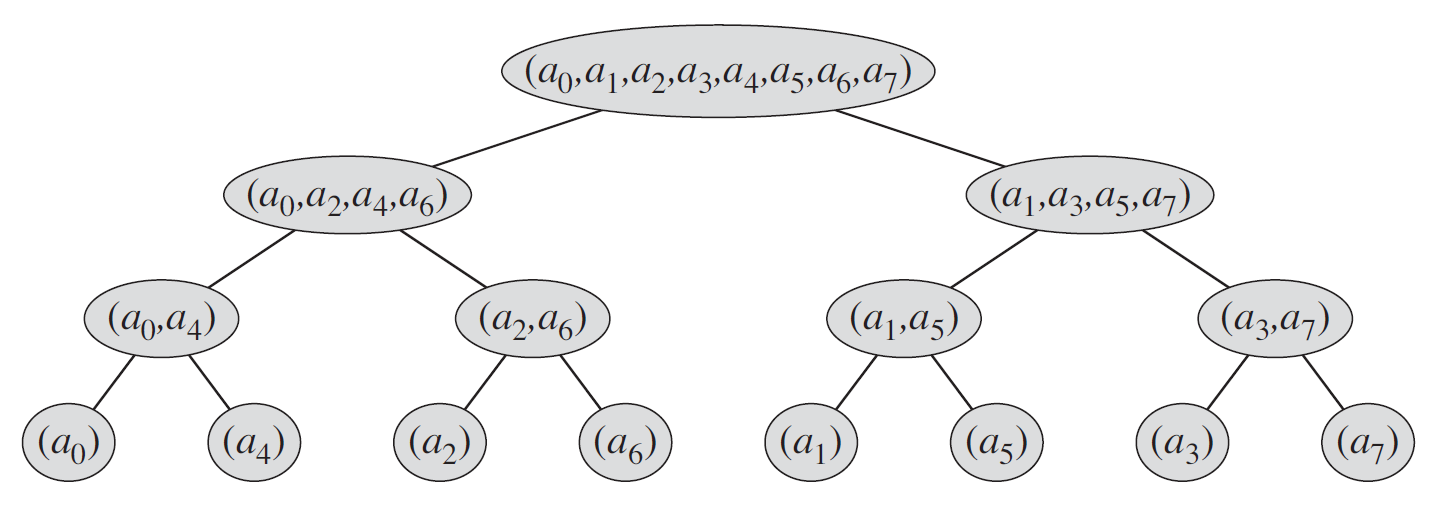
\includegraphics[scale=0.4]{./FFT/pic/pic3.PNG}
    \caption{n = 8 일때,recursive시 분할되는 원소들}
\end{figure}

\begin{figure}[h!]
    \centering
    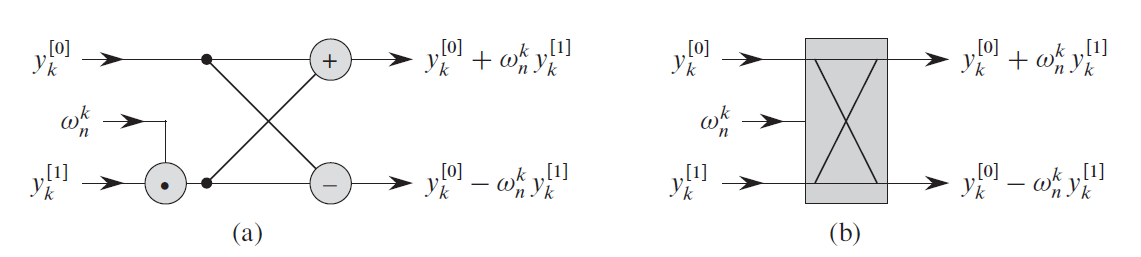
\includegraphics[scale=0.5]{./FFT/pic/pic4.PNG}
\end{figure}


\begin{figure}[h!]
    \centering
    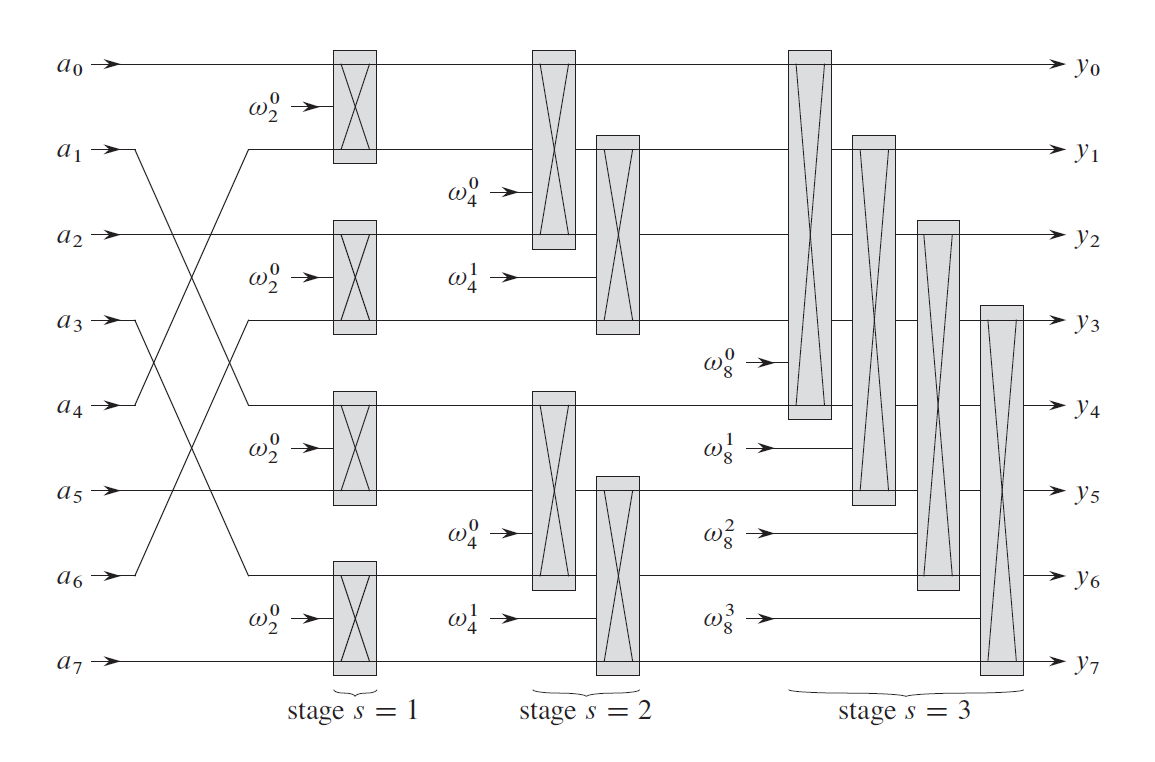
\includegraphics[scale=0.5]{./FFT/pic/pic5.PNG}
    \caption{n = 8의 iterative-FFT 수행}
\end{figure}



\begin{lstlisting}[style = CStyle]
ITERATIVE-FFT(a)
    BIT-REVERSE-COPY(a, A)
    n = a.length // n is a power of 2
    for s = 1 to lg n
        m = 2^s
        w_m = e^{2pi i/m}
        for k = 0 to n-1 by m
            w = 1
            for j = 0 to m/2 -1
                t = w A[k+ j + m /2]
                u = A[k + j]
                A[k + j] = u + t
                A[k+ j + m /2] = u - t
                w = w_m
    return A
\end{lstlisting}

\begin{lstlisting}[style = CStyle]
BIT-REVERSE-COPY(a, A)
    n = a.length
    for k = 0 to n - 1
        A[rev(k)] = a_k
\end{lstlisting}


마지막으로 parallel 알고리즘으로 바꾸는것이다.


\begin{thebibliography}{}
    \bibitem{reference1}
    Thomas H. Cormen, Charles E. Leiserson, Ronald L. Rivest, and Clifford Stein. Introduction to Algorithms, Second Edition. MIT Press and McGraw-Hill, 2001. ISBN 0-262-03293-7.
\end{thebibliography}